Theory

\section{Key Terms}
Words to define: 
•	Citizen Science \cite{tweddle_guide_2012}
•	Stakeholders - people who live, commute or work in coastal Trondheim - people with awareness of the 4 places coastline
•	Resilience - cutter
•	Place (& space) - Massey
•	Awareness (vs knowledge vs perception)
•	Vulnerability – Lujala / Lein / Setten 

Words to explain:
•	Disaster-> Sea level extreme event
•	High water
•	tide
•	Uplift
•	Storm surge
•	1 in 20 year storm surge

\section{Projecting Resilience of Place}
Key theories:
•	DROP cutter
•	Social systems as what defines resilience
•	Projected resilience as dynamic process which influences outcomes (i.e. resilience as measured post disaster). 
•	Cutter et al 2008
•	Cutter 2020 
•	Moser et al 2019 

\section{Defining Resilience} 
Resilience is here considered as the ability to return to normality as quickly as possible after disaster this is in line with (Cutter, 2019:Löw, 2019).

"present does not define future resilience, but it does influence it. Resilience as dynamic and dependent on 3 changing systems -natural, social & technological
" \cite{cutter_community_2020} views of resilience.

Sea Level Extremes can cause disaster, but this is not necessarily the case. A sea level extreme thus can be viewed as a possible disaster which is referred to here as an event. 

""Resilience is the ability of a social system to respond and recover from disasters and includes those inherent conditions that allow the system to absorb impacts and cope with an event, as well as post-event, adaptive processes that facilitate the ability of the social system to re-organize, change, and learn in response to a threat" "Vulnerability is the pre-event, inherent characteristics or qualities of social systems that create the potential for harm. Vulnerability is a function of the exposure (who or what is at risk) and sensitivity of system (the degree to which people and places can beharmed" " \cite{cutter_place-based_2008}


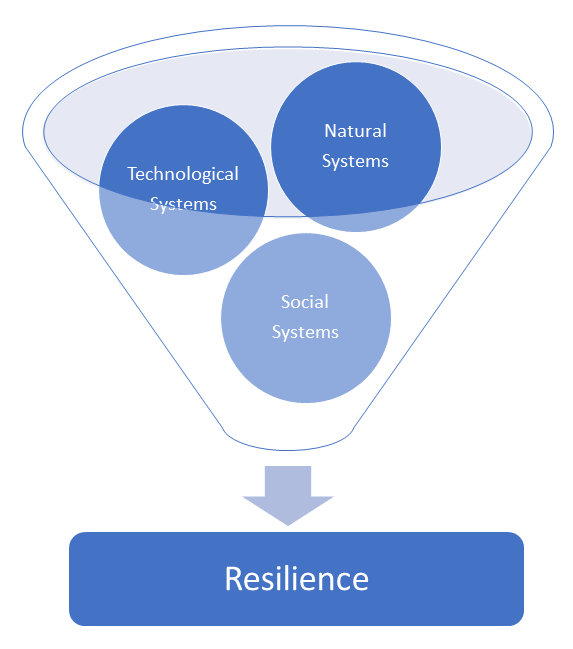
\includegraphics[scale=1.1]{fig_theory/resilience model .png}
\mbox{}\\[6pc]

Resilience is an ongoing dynamic process. When discussing resilience in this thesis we are discussing projected resilience. Hence what is the projected ability to return to normality as quickly as possible after an sea level extreme event. 
 
Focusing on place based resilience and including community and institutions under the social system aspect
Rather than using community resilience in its place-based approach as commonly conceptualised in Norway both in National and local policy documents and by “layperson” (Räsänen et al 2020). Especially as highlighted by (Räsänen et al 2020) that how useful current place -based metirics are for measuring community resilience and that there is need for other techniques. Hence don’t ignore community but place it under social systems. 
•	Place based resilience vs community resilience
•	What they are why they differ and why I am using place based resilience

\section{Space and Place} 
“According to Massey (2005), space is the dimension of simultaneity and is part of space-time.
Space is considered as the dimension of things being and being at the same time. If we
consider time as things occurring one after the other, then space is when things occur
simultaneously. The network of relations and connections within space reflects the power
networks that operate within societies. Space is both socially constructed and in constant
negotiation: these negotiations are in turn affected by power (Allen, 2002). This definition of
space is relevant in public, private and virtual spaces (Massey, 2005).” From geog3517 exam paper

The four chosen areas are a combination of public and private space, however the edge of the water itself is usually considered public space. There is also space allocated to groups whose membership is very open to the majority of the public, but it still creates feelings of in-place vs out-of-place


“An important aspect in the continuous power ridden negotiation of place is the defining of who is “in place” or “out of place” (Allen, 2002; Anderson, 2015; Sharp, 2000). “In place” can be considered
those who belong within a specific locale. The traces of place influence what is considered
allowable uses of the place and even who can use it (Anderson, 2015). This cultural ordering
and geographical bordering can also create a group who are “out of place”. This occurs when
the traces left indicate that who they are and their actions are not welcome – in other words
they do not belong (Anderson, 2015).” From geog3517 term paper

\section{Awareness}
To understand level of resilience of the area required an understanding of the awareness of the people who interact with and define the four chosen places. (Considering place as an assemblage of traces from the historical and global to the local and present, these traces combine to make place (Anderson, 2015; Massey, 2005). – from GEOG3517 exam paper)

An individual’s ability to rank their level of awareness about a subject is a long investigated and debated topic. It is generally preferable to allow them to display their level of awareness rather than ask them on a sliding scale how aware they are. Especially when trying to explore knowledge which may have previously been seen as lesser in comparison to academic knowledge. 
To determine awareness level three questions were set in the survey used. These questions were designed to be simple and quick to answer in a format which would allow the author to analyse awareness about sea level extremes in the present and future along with general knowledge of the sea. 
Awareness about tide level, current risk of storm surges, past resilience to storm surges and future resilience to storm surges was investigated. Further information of how different question techniques and formats were trialled, and the influence of the decided questions format can be found in the Method section. The choice which format method to use while asking about sea level changes is likely to have an influence on how participants perceive this change. For example considering change as metres in height vs area of land influenced may results in different perceptions of the changing risks and potential impacts.  By sticking firmly in the realm of historical fact and scientific models with these questions there has been an attempt to investigate awareness of SLEs rather than perception. 

•	Local knowledge vs awareness
•	Local knowledge and resilience 

\section{Social Systems impacting Resilience}
community resilience as key aspect of social systems
local knowledge is part of that

\section{Technological Systems}

\section{Natural Systems }
SLE = WAVE + SEA LEVEL + TIDE + STORM SURGES + land movement

Storm Surge
“Storm surges are high water levels in the sea that occur during spring tides in combination with special weather conditions such as low air pressure and strong onshore winds.” According to the kommune (Einar Aassved Hanssen, Marianne Langedal, 2013) – stormflo = storm surge
“Safety against floods and storm surges is regulated by safety classes based on the
largest nominal annual probability. Flood sizes are usually stated with a number of
years of repetition intervals. The recurrence interval indicates how often a flood or
storm surge of the same magnitude occurs on average over many long years. A flood
with a recurrence interval of 200 years, also called a 200-year flood, occurs on average
every 200 years. Each year, the probability of a 200-year flood is equal to 1/200, ie 0.5 percent.
This does not exclude that one can get two 200-year floods at short intervals.
Calculation of recurrence intervals for floods and storm surges is based on historical
observations, and measurement of water flow or water level.”
Building technical regulations (TEK17) with guidance Chapter 7 Safety against natural stresses
